\documentclass{beamer}

\usepackage[latin1]{inputenc}
\usepackage{amsmath}
\usepackage{amssymb}

\usecolortheme[RGB={239,165,80}]{structure}
\useoutertheme{infolines}
\usetheme[height=10mm]{Rochester}
\setbeamertemplate{items}[circle]
\setbeamertemplate{blocks}[rounded][shadow=true]
\setbeamertemplate{navigation symbols}{}

\title[Degrees of belief]
      {An introduction to Bayesian probabilities and their application}

\author{Kieran Gorman}
\institute{Xero}
\date{2015}
\begin{document}

\begin{frame}
  \titlepage
\end{frame}


\begin{frame}{Probability}

  \begin{itemize}
    \setlength\itemsep{1em}
    \item How 'likely' is the occurrence of a certain event?
    \item Traditionally 'frequentist'.
    \item The limit given relative observed frequency.
    \item That is, having observed $P(x) \approx \frac{n_x}{n_t}$ we
      might deduce that $P(x) = \lim_{x\to\infty} \frac{n_x}{n_t}$
    \item In the frequentist model, a hypothesis is a well defined
      proposition (i.e. certainly true or certainly false).
  \end{itemize}

\end{frame}

\begin{frame}{Probability cont.}

  \begin{center}
    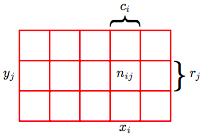
\includegraphics[scale=0.5]{pgrid}
  \end{center}

  \begin{itemize}
    \item Joint: $P(X = x_i, Y = y_j) = \frac{n_{ij}}{N}$
    \item Sum rule: $P(X = x_i) = \sum_{j=1}^{L}P(X = x_i, Y = y_j)$
    \item Conditional: $P(Y = y_j | X = x_i) = \frac{n_{ij}}{c_i}$ \\
      $P(X = x_i, Y = y_j) = \frac{n_{ij}}{N} = \frac{n_{ij}}{c_i}
      \cdot \frac{c_i}{N}$
    \item Product rule: $P(X = x_i, Y = y_j) = P(Y = y_j | X = x_i) \cdot
      P(X = x_i)$
  \end{itemize}

  \begin{center}
    {\tiny
      This also hold for continuous variables, as probability
      densities, just replace $\sum$ with $\int$
    }
  \end{center}

\end{frame}

\begin{frame}{Bayes Theorem}

  It's just an application of the sum and product rules.


  \begin{align}
    P(X, Y) &= P(Y, X) \nonumber \\
    P(Y|X) \cdot P(X) &= P(X|Y) \cdot P(Y) \nonumber \\
    P(Y|X) &= \frac{P(X|Y) \cdot P(Y)}{P(X)} \nonumber
  \end{align}

  We're not quite at actual Bayesian probabilities, but we can
  immediately begin to apply Bayes theorem in a classification problem.

\end{frame}

\begin{frame}{Na\"ive Bayes Classifier}

  Apply Bayes theorem, along with a strong independence assumption
  (this is what makes it 'na\"ive').

  \begin{align}
    p(C_k, x_1, \ldots, x_n) &= p(C_k)p(x_1, \ldots, x_n | C_k)
    \nonumber \\
    &= p(C_k)p(x_1|C_k)p(x_2, \ldots, x_n | C_k, x_1) \nonumber \\
    &= p(C_k)p(x_1|C_k)p(x_2|C_k, x_1)p(x_3,\ldots,c_n|C_k,x_1,x_2)
    \nonumber \\
    &= p(C_k)p(x_1|C_k)p(x_2|C_k,x_1)\ldots p(x_n|C_k,x_1,\ldots,
    x_{n-1}) \nonumber
  \end{align}

  Now assume all of the values in the input vector are independent of
  one another, meaning $P(A|B, C) = P(A|B) \cdot P(A|C)$. In our case
  it means that $p(x_i | C_k, x_j, x_k) = p(x_i | C_k)$.

\end{frame}

\begin{frame}{Na\"ive Bayes Classifier cont.}
  So, applying Bayes theorem we get

  \begin{align}
  P(C_k|x_1, \ldots, x_n) &\propto p(C_k) p(x_1,\ldots,x_n | C_k)
  \nonumber \\
  &\propto p(C_k) p(x_1 | C_k) p(x_2 | C_k) \ldots p(x_n | C_k)
  \nonumber \\
  &\propto p(C_k)\prod_{i=1}^{n}P(x_i | C_k) \nonumber
  \end{align}

  That is, the probability of labelling an input instance with a
  certain class is simply the probability of that class, multiplied by
  the likelihood that instance appearing in that class based on what
  we've seen already.


  {\tiny
    This assumption is clearly false in almost all interesting
    cases, however in general corpus is king. See ``unreasonable
    effectiveness of data'', from Norvig at google.
  }

\end{frame}

\begin{frame}{Contrived demonstration}

  Demo.

\end{frame}

\begin{frame}{A Bayesian approach}

  We can interpret Bayes theorem as:

  \begin{align}
    p(A|B) &= \frac{p(B|A) \cdot p(A)}{p(B)} \nonumber \\
    &\propto p(B|A) \cdot p(A) \nonumber \\
    posterior &\propto likelihood \cdot prior \nonumber
  \end{align}

  We can see that by counting frequencies, we are fixing our
  probability estimator to one that maximises likelihood for computing
  $p(x)$.

  In contrast Bayesian probabilities factor in our prior degree of
  belief more explicitly by dealing in probability distributions.

\end{frame}

\begin{frame}{A Bayesian approach cont.}

  \begin{itemize}
    \item Consider for example events we have a degree of belief in
      occurring, but we can't readily measure (say, the state of the
      polar ice caps at the turn of the next century).
    \item Bayesian probabilities are sometimes called ``a logical
      approach to probabilities'' and can be derived from Cox's axioms
      (i.e. ``degrees of belief'') for example.
    \item In frequentism we have a fixed probability and then error
      bars on that probability representing multiple possible
      datasets.
    \item In Bayesianism, we have a single (observed) dataset, and
      then an ``error'' in our probability by instead representing it
      as a distribution.
  \end{itemize}

\end{frame}

\begin{frame}{A brief digression into neural networks}

  A brief digression: neural networks.

  \begin{itemize}
  \item For this talk, considered supervised learners.
  \item Given an input vector, produce an output vector.
  \item Commonly, choose scalar with greatest value in output vector as
    classification.
  \item Train posterior classification through combination of input
    probability and learned weightings.
  \item Essentially just layered logistic regression, with training.
  \end{itemize}

\end{frame}

\begin{frame}{Logistic wha?}

  Enter, the perceptron.

  \begin{center}
    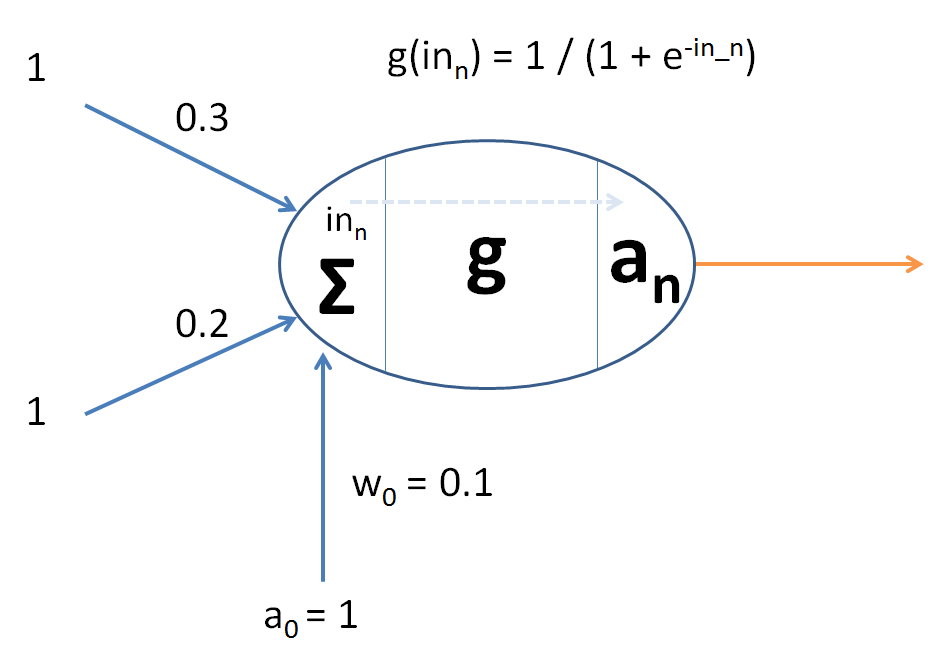
\includegraphics[scale=0.4]{ptron}
  \end{center}

\end{frame}

\begin{frame}{Mulitlayered}
  Exeunt perceptron, enter the multi-layer perceptron:

  \begin{center}
    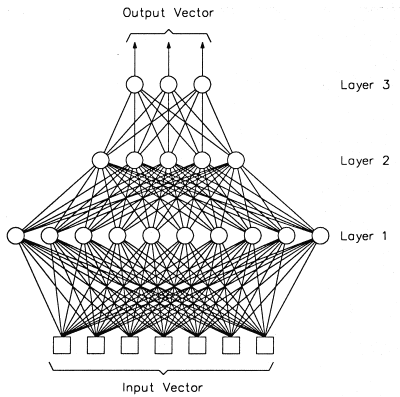
\includegraphics[scale=0.4]{multi}
  \end{center}

\end{frame}

\begin{frame}{Gradient descent search}
  Now, the question is: how do we choose good values for the
  weightings?

  \begin{itemize}
    \item Need to have some measure of accuracy, ``fitness function''
      (e.g. least squared error, minimal mis-classification)
    \item Given the notion of ``distance'', we can propagate updates
      to our weights proportional to distance (i.e. being very
      incorrect has a much greater effect than being only slightly
      off).
    \item Called, unsurprisingly, backpropagation algorithm and uses
      gradient descent search to find minima.
    \item General idea: provide sets of input vectors with known
      outputs, iterate search until we reach a termination condition
      (perhaps just $n$ iterations, or net movement in error per epoch
      etc.)
    \item Seems somewhat similar to Bayes theorem (prior, likelihood,
      evidence all contribute to a posterior), but the probabilities
      themselves are still maximum likelihood (i.e. frequentist).
  \end{itemize}
\end{frame}

\end{document}
